\scanpage{56}
% archive sheet number: 55

\[ (\nu_{s_1}-1)+(\nu_{s_2}-1)\ldots+(\underbrace{\nu_{s_n}}_{\nu_{s_0}}-1)\unsure{''} \]

\figure{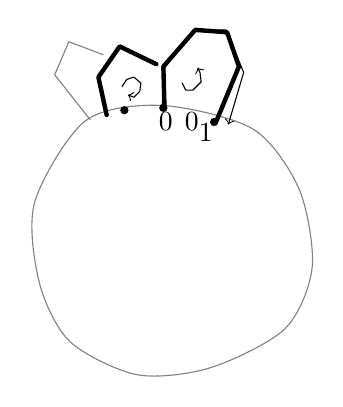
\begin{tikzpicture}[x=0.015cm,y=-0.015cm,line cap=round,line join=round]
\draw[gray,thin] plot[smooth cycle] coordinates {(95,93) (160,80) (237,100) (276,151) (287,217) (264,269) (201,302) (139,308) (82,280) (56,230) (52,162)};
\draw[gray,thin] (99,92)--(69,54)--(81,26)--(110,37);
\draw[->] (160,81)--(162,48)--(187,17)--(214,16)--(229,52)--(216,96);
\draw[line width=1.6pt] (162,83)--(161,47)--(188,16)--(215,18)--(225,47)--(206,93);
\draw[line width=1.6pt] (113,88)--(106,56)--(124,30)--(155,45);
\draw[->] (126,64)--(130,58)--(136,56)--(142,61)--(141,68)--(136,73)--(131,71);
\draw[->] (177,61)--(180,67)--(186,67)--(193,60)--(192,52)--(190,48);
\fill[black] (128,84) circle [radius=1.5pt];
\fill[black] (161,82) circle [radius=1.5pt];
\fill[black] (204,94) circle [radius=1.5pt];
\node at (163,94) {$0$};
\node at (185,94) {$0$};
\node at (197,103) {$1$};
\end{tikzpicture}}

\figure{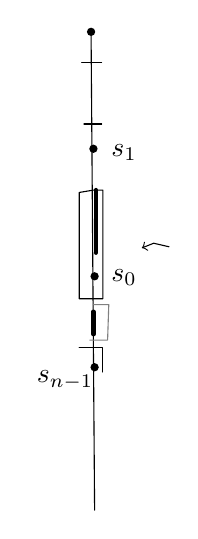
\begin{tikzpicture}[x=0.015cm,y=-0.015cm,line cap=round,line join=round]
\draw[thin] (26,0)--(29,405);
\draw[thin] (18,26)--(35,26);
\draw[thin] (20,78)--(35,78);
\fill[black] (26,0) circle [radius=1.5pt];
\fill[black] (28,99) circle [radius=1.5pt];
\fill[black] (29,207) circle [radius=1.5pt];
\fill[black] (29,284) circle [radius=1.5pt];
\draw[thin] (27,134)--(36,134)--(36,226)--(16,226)--(16,136)--(28,134);
\draw[line width=1.6pt] (30,134)--(30,187);
\draw[gray,thin] (28,231)--(41,231)--(40,261)--(25,261);
\draw[line width=1.6pt] (28,237)--(28,256);
\draw[thin] (16,267)--(36,267)--(36,288);
\node at (54,102) {$s_1$};
\node at (54,208) {$s_0$};
\node at (4,295) {$s_{n-1}$};
\draw[->] (92,182)--(79,179)--(69,183);
\end{tikzpicture}}

\[ \begin{aligned}
l_s&=\deleted{\unsure{\ell}}n-\nu_s\\
l_a&=\deleted{\unsure{\ell}}n-1-(\nu_s-1)-(\nu_t-1)\\
&=n\deleted{\unsure{+}}\unsure{-}(\nu_s+\nu_t-1)=(n-\nu_s)-(\nu_t-1)\\
l_s-l_a&=\nu_t-1\quad\deleted{\unsure{=2|=1}}\\
\chi_{2n}(s)&=\sum_{\substack{s\text{ sommets}\\\text{sur }D_i}}(\nu(s)-1)=n-1
\end{aligned} \]

\margin{multiplicité du sommet \quad $\mathbb Z/N\mathbb Z$}

\[ \lambda(t)=\widetilde\rho_p(t)=(-1)^p(t-\chi_p) \]

ici $p=2n$ donc $(-1)^p=+1$

\[ \deleted{\unsure{\beta}} \quad \deleted{\text{il faut}}\quad \lambda(t)=\deleted{\unsure{a}}t-\chi_{2n}=t-(n-1) \]

\uline{NB}

\[ \begin{aligned}
\rho_p(t)&=\sigma_{p-1}\ldots\sigma_0(t)=\deleted{(-1)^{p-1}(\chi_p-t)}\inserted{(-1)^p(t-\chi_p)}\\
&\deleted{=(-1)^p t+(-1)^{p-1}\chi_p}
\end{aligned} \]

Passage de $F_p$ à $F_0$ se fait par $t\longleftarrow\deleted{\unsure{t}}\ t$ \deleted{(\unsure{en effet}, \illegible{3})}

\[ \underbrace{\sigma_{p-1}\sigma_p\ldots\sigma_0}_{\rho_p(t)}(t)=(-1)^{p-1}\ldots \]

\figure{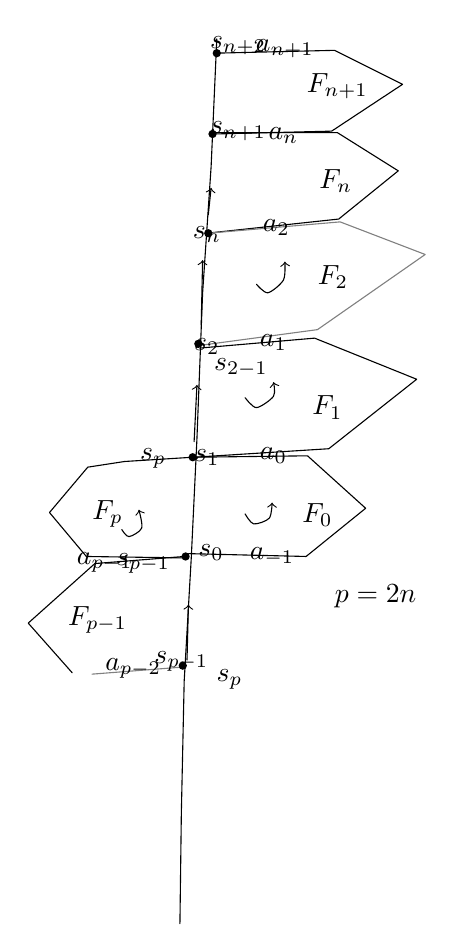
\begin{tikzpicture}[x=0.018cm,y=-0.018cm,line cap=round,line join=round]
\draw[thin] (125,0)--(121,90)--(115,179)--(111,282)--(107,366)--(102,453)--(100,546)--(99,624);
\draw[thin] (124,10)--(208,8)--(256,32)--(206,65)--(123,67);
\draw[thin] (122,66)--(210,66)--(253,93)--(211,127)--(118,137);
\draw[gray,thin] (119,137)--(212,129)--(272,152)--(196,205)--(114,216);
\draw[thin] (113,218)--(194,211)--(266,240)--(204,289)--(109,295);
\draw[thin] (109,295)--(189,294)--(230,331)--(188,365)--(105,363);
\draw[thin] (108,295)--(60,298)--(34,302)--(7,334)--(33,365)--(101,366);
\draw[thin] (102,365)--(39,370)--(-8,412)--(23,447);
\draw[gray,thin] (37,448)--(101,443);
\draw[->] (104,438)--(105,399);
\draw[->] (109,284)--(111,244);
\draw[->] (114,202)--(115,156);
\draw[->] (119,124)--(121,105);
\fill[black] (125,10) circle [radius=1.5pt];
\fill[black] (122,67) circle [radius=1.5pt];
\fill[black] (119,137) circle [radius=1.5pt];
\fill[black] (112,215) circle [radius=1.5pt];
\fill[black] (108,295) circle [radius=1.5pt];
\fill[black] (103,365) circle [radius=1.5pt];
\fill[black] (101,442) circle [radius=1.5pt];
\node at (140,5) {$s_{n+2}$};
\node at (173,7) {$a_{n+1}$};
\node at (210,33) {$F_{n+1}$};
\node at (140,65) {$s_{n+1}$};
\node at (172,68) {$a_n$};
\node at (209,100) {$F_n$};
\node at (118,138) {$s_n$};
\node at (167,133) {$a_2$};
\node at (207,168) {$F_2$};
\node at (118,217) {$s_2$};
\node at (142,232) {$s_{2-1}$};
\node at (165,214) {$a_1$};
\node at (203,260) {$F_1$};
\node at (118,295) {$s_1$};
\node at (80,296) {$s_p$};
\node at (165,294) {$a_0$};
\node at (196,336) {$F_0$};
\node at (48,335) {$F_p$};
\node at (73,370) {$s_{p-1}$};
\node at (121,362) {$s_0$};
\node at (164,365) {$a_{-1}$};
\node at (46,369) {$a_{p-1}$};
\node at (41,410) {$F_{p-1}$};
\node at (66,444) {$a_{p-2}$};
\node at (100,439) {$s_{p-1}$};
\node at (134,452) {$\deleted{\unsure{s_p}}$};
\node at (237,393) {$p=2n$};
\draw[->] plot[smooth] coordinates {(58,346) (63,351) (72,345) (70,332)};
\draw[->] plot[smooth] coordinates {(145,335) (151,342) (162,338) (164,327)};
\draw[->] plot[smooth] coordinates {(145,253) (153,260) (165,252) (165,242)};
\draw[->] plot[smooth] coordinates {(153,173) (161,179) (172,170) (173,157)};
\end{tikzpicture}}

\figure{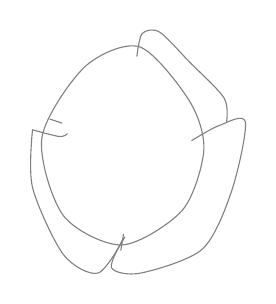
\begin{tikzpicture}[x=0.017cm,y=-0.017cm,line cap=round,line join=round]
\draw[gray,thin] plot[smooth cycle] coordinates {(16,79) (48,26) (89,11) (126,51) (137,88) (121,133) (76,159) (32,137)};
\draw[gray,thin] plot[smooth] coordinates {(9,73) (29,78) (35,76)};
\draw[gray,thin] plot[smooth] coordinates {(9,73) (9,116) (32,166) (58,180) (78,153)};
\draw[gray,thin] plot[smooth] coordinates {(77,154) (68,176) (90,180) (136,162) (158,118) (168,67) (148,70) (128,81)};
\draw[gray,thin] plot[smooth] coordinates {(154,67) (152,49) (126,22) (104,0) (91,1) (87,18)};
\draw[gray,thin] (22,65)--(31,68);
\draw[gray,thin] (77,151)--(75,163);
\end{tikzpicture}}

\figure{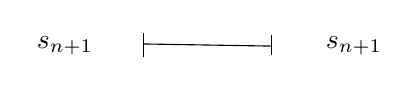
\begin{tikzpicture}[x=0.027cm,y=-0.027cm,line cap=round,line join=round]
\draw[thin] (0,2)--(60,3);
\draw[thin] (0,-3)--(0,8);
\draw[thin] (60,-2)--(60,7);
\node at (-37,3) {$s_{n+1}$};
\node at (99,3) {$s_{n+1}$};
\end{tikzpicture}}

\diagram{\begin{tikzcd}[ampersand replacement=\&,column sep=huge]
P(F_n) \arrow[r,"\sigma_{a_n}"] \arrow[d,phantom,"\unsure{\wr}" description] \& P(F_{n+1}) \arrow[d,phantom,"\unsure{\wr}" description]\\
\mathbb Z/N\mathbb Z \arrow[r,"\sigma_n"] \arrow[u,phantom,"\varphi_n"'] \& \deleted{\unsure{\mathbb Z}}\mathbb Z/N\mathbb Z \arrow[u,phantom,"\varphi_{n+1}"]
\end{tikzcd}}

$\sigma_n$ \quad \unsure{a)} respecte la structure polygonale

b) renverse l'orientation

c) transforme $\underbrace{\varphi_n^{-1}(s_{n+1})}_{l_n}$ en $\underset{\substack{\Vert\\0}}{\varphi_{n+1}^{-1}(s_{n+1})}$

\[ \text{donc}\quad \sigma_n(t)=l_n-t \]

\[ \begin{aligned}
\sigma_0(t)&=l_0-t\\
\sigma_1(t)&=l_1-t &\sigma_1\sigma_0(t)&=l_1-(l_0-t)=l_1-l_0+t\\
\sigma_2(t)&=l_2-t &\sigma_2\sigma_1\sigma_0(t)&=l_2-l_1+l_0-t
\end{aligned} \]

\[ \begin{aligned}
(\underbrace{\overbrace{\sigma_n\deleted{\unsure{\sigma}}\sigma_{n-1}\ldots\sigma_0}^{n+1\ \text{facteurs}}}_{\rho_{n+1}})(t)&=l_n-l_{n-1}-\ldots+(-1)^n l_0+(-1)^{n+1}t\\
&=(-1)^n(\chi_{n+1}-t)=(-1)^{n+1}(t-\chi_{n+1})\\
\text{où}\quad \chi_{n+1}&=\underbrace{l_0\deleted{+}\unsure{-|+}l_1-\ldots+(-1)^n l_n}_{n+1\ \text{termes}}
\end{aligned} \]
